\clearpage
\subsection{MSVC: x86 + \olly}
\index{\olly}

\RU{Тут даже проще}\EN{Things are even simpler here}:

\begin{figure}[H]
\centering
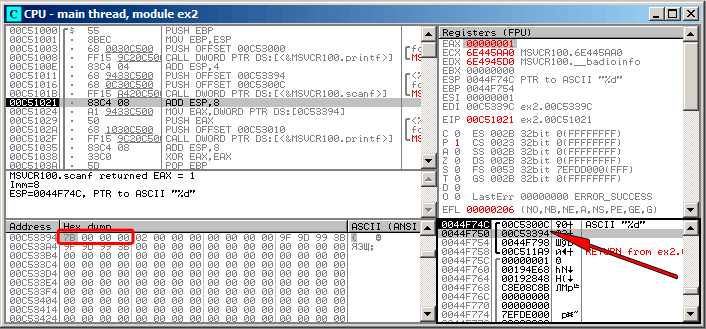
\includegraphics[scale=\FigScale]{patterns/04_scanf/2_global/ex2_olly_1.png}
\caption{\olly: \RU{после исполнения \scanf}\EN{after \scanf execution}}
\label{fig:scanf_ex2_olly_1}
\end{figure}

\RU{Переменная хранится в сегменте данных}\EN{Variable is located in the data segment}.
\RU{Кстати, после исполнения инструкции \PUSH (заталкивающей адрес $x$) адрес появится в стеке, и на этом
элементе можно нажать правой кнопкой, выбрать ``Follow in dump''}\EN{By the way, after 
\PUSH instruction (pushing $x$ address) is executed, the address
will appear in stack, and it is possible to right-click on that element and select ``Follow in dump''}.
\RU{И в окне памяти слева появится эта переменная}\EN{And the variable will appear in the memory window
at left}.

\RU{После того как в консоли введем 123, здесь появится}\EN{After we enter 123 in the console,} 
\TT{0x7B}\EN{ will appear here}.

\RU{Почему самый первый байт это}\EN{But why the very first byte is} \TT{7B}?
\RU{По логике вещей, здесь должно было бы быть}\EN{Thinking logically, a} \TT{00 00 00 7B}\EN{ should be
there}.
\RU{Это называется}\EN{This is what called} \gls{endianness}, \RU{и в x86 принят формат}\EN{and} 
\IT{little-endian}\EN{ is used in x86}.
\RU{Это означает что в начале записывается самый младший байт, а заканчивается самым старшим байтом}
\EN{This mean that lowest byte is written first, and highest written last}.
\RU{Больше об этом}\EN{More about it}: \ref{sec:endianness}.

\RU{Позже, из этого места в памяти, 32-битное значение загружается в \EAX и передается в}
\EN{Some time after, 32-bit value from this place of memory is loaded into \EAX and passed into} \printf.

\RU{Адрес переменной $x$ в памяти}\EN{$x$ variable address in the memory is} \TT{0x00C53394}.

\clearpage
\RU{В \olly{} мы можем посмотреть карту памяти процесса (Alt-M) и увидим что этот адрес
внутри PE-сегмента \TT{.data} нашей программы}\EN{In \olly we can see process memory map (Alt-M)
and we will see that this address is inside of \TT{.data} PE-segment of our program}:

\begin{figure}[H]
\centering
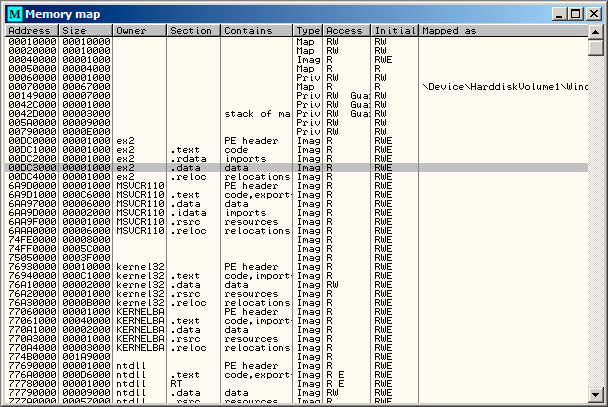
\includegraphics[scale=\FigScale]{patterns/04_scanf/2_global/ex2_olly_2.png}
\caption{\olly: \RU{карта памяти процесса}\EN{process memory map}}
\label{fig:scanf_ex2_olly_2}
\end{figure}
